\section{The kernel-free boundary intergral method} \label{KFBI}
% \subsection{Introduction of KFBI-CPU method}
Suppose $\Omega$ is a bounded irregular and complex domain in $R^2$ or $R^3$ whose boundary $\Gamma = \partial \Omega$ is at least twice continuously differentiable. Let $u(\mathbf{x})$ be an unknown function of $\mathbf{x} \in \mathbf{R}^{d}(d=2, or ~3)$. Assuming $g_{D}(\mathbf{x})$ and $f(\mathbf{x})$ are known function of $\mathbf{x}$  with sufficient smoothness. $\partial_{\mathbf{n}}u(\mathbf{x})$ denotes the normal derivative of $u(\mathbf{x})$ on the boundary, where $\mathbf{n}$ denotes the unit outward normal on $\Gamma$. For simplicity of description, we introduce the KFBI method for the modified Helmholtz equation subject to the Dirichlet boundary condition. 

Consider the modified Helmholtz equation 
\begin{equation}
    \Delta u(\mathbf{x})-\kappa u(\mathbf{x})=f(\mathbf{x}), \quad \text { in } \Omega,
    \label{one_GPU:modified_helmholtz}
\end{equation}
subject to Dirichlet boundary condition 
\begin{equation}
    u(\mathbf{x}) = g_{D}(\mathbf{x}), \quad \text{ on }\Gamma.
    \label{one_GPU:dirichlet_boundary}
\end{equation}

Here, $\kappa$ is assumed to be a positive constant for the modified Helmholtz equation in this paper by default.

\subsection{Boundary integral equation}
As shown in Fig.\,$\ref{kfbi domain}$, to solve the boundary value problem above by the KFBI method, we first embed the irregular domain $\Omega$ into a larger rectangle domain $\mathcal{B} = \Omega \cup \Omega^{c}$. 

\begin{figure}[htpt!]
    \centering
    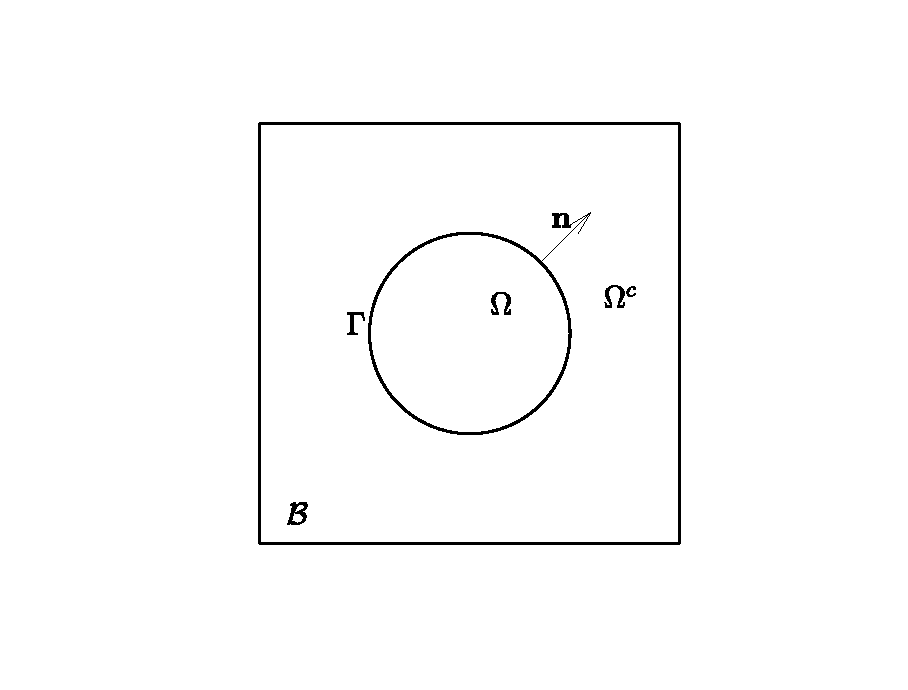
\includegraphics[width = 0.8\linewidth]{figure/one_gpu_kfbi1.eps}
    \caption{KFBI computation domain}
    \label{kfbi domain}
\end{figure}

According to the standard BIM\cite{aliabadi2011boundary,yu2002natural}, let $G(\mathbf{x}, \mathbf{y})$ be  Green's function on the rectangle $\mathcal{B}$ associated with the elliptic PDE $\eqref{one_GPU:modified_helmholtz}$, which satisfies for $\mathbf{y} \in \mathcal{B}$,
\begin{align}
\triangle G(\mathbf{x}, \mathbf{y})-\kappa G(\mathbf{x}, \mathbf{y}) &= \delta(\mathbf{x}-\mathbf{y}), \quad \mathbf{x} \in \mathcal{B}, \\
G(\mathbf{x}, \mathbf{y}) &=0 \quad \mathbf{x} \in \partial \mathcal{B},
\end{align}
where $\delta(\mathbf{x} - \mathbf{y})$ is the Dirac delta function. Let $\mathbf{n}_{\mathbf{y}}$ be the unit outward normal vector at point $\mathbf{y}\in \Gamma$, and $\varphi$ be the density function. We first define the double layer boundary integral and volume integral by
\begin{align}
(W \varphi)(\mathbf{x}) := \int_{\Gamma} \frac{\partial G(\mathbf{y}, \mathbf{x})}{\partial \mathbf{n}_{\mathbf{y}}} \varphi(\mathbf{y}) d s_{\mathbf{y}}, \quad & \text { for } \mathbf{x} \in \Omega \cup \Omega^{c},\label{one_GPU:double} \\
(Yf)(\mathbf{x}) := \int_{\Omega} G(\mathbf{y}, \mathbf{x})f(\mathbf{y}) d\mathbf{y}, \quad & \text{ for } ~\mathbf{x} \in \mathbf{R}^{2}.
    \label{one_GPU:volume}
\end{align}

% Let $\psi$ be the density function, and define the single layer boundary integral by
% \begin{equation}
% (V \psi)(\mathbf{x}) := \int_{\Gamma} G(\mathbf{y}, \mathbf{x}) \psi(\mathbf{y}) d s_{\mathbf{y}} ~\text { for } ~\mathbf{x} \in \Omega \cup \Omega^{c}  \label{single}
% \end{equation}

Thanks to the symbols and properties of the involved potential and volume integral, the Dirichlet BVP $\eqref{one_GPU:modified_helmholtz}$-$\eqref{one_GPU:dirichlet_boundary}$ can be reformulated as a Fredholm boundary integral equation of the second kind\cite{kress1989linear,hsiao2008boundary} by Green’s third identity.
\begin{equation}
    \frac{1}{2}\varphi (\mathbf{x}) + (W\varphi)(\mathbf{x}) + (Yf)(\mathbf{x}) = g_{D}(\mathbf{x}), \quad \mathbf{x} \text { on } \Gamma. \label{one_GPU:second_fredholm}
    % 
    % g_D(\mathbf{x})  =(W \varphi)^{+}(\mathbf{x})+(Y f)^{+}(\mathbf{x}), \quad & \mathbf{x} \in \Gamma  \label{One_GPU:boundary_dirichlet}
\end{equation}

The solution $u(\mathbf{x})$ to the Dirichlet BVP $\eqref{one_GPU:modified_helmholtz}$-$\eqref{one_GPU:dirichlet_boundary}$ is given by 
\begin{equation}
    u(\mathbf{x}) = (W\varphi)(\mathbf{x}) + (Yf)(\mathbf{x}), \quad \mathbf{x} \in \Omega. \label{One_GPU:fredholm_dirichlet} \\
\end{equation}

Let $M>2$ be an integer and $\left\{\mathbf{x}_j\right\}_{j=0}^{\mathrm{M}}$ be a set of quasi-uniformly spaced points on the domain boundary $\Gamma$ so that each curve segment $\widetilde{\mathbf{x}_i \mathbf{x}_{i+1}}(i=0,1, \cdots, M-1)$ has nearly equal length. Numerically, the boundary integral equation $\eqref{one_GPU:second_fredholm}$ can be solved by the Richardson iteration: given an initial guess $\varphi_{0}(\mathbf{x}_{m})$, for $k \in \left\{0, 1, 2, 3, \cdots\right\}, m \in \left\{0, 1, 2, \cdots, M\right\}$, do as follows
\begin{align}
    % \hat{g}_{D}(\mathbf{x}) = g_{D}(\mathbf{x}) - (Yf)(\mathbf{x}), & \quad \mathbf{x} \in \Gamma, \\
    u_{k}^{+}(\mathbf{x}_{m}) = \frac{1}{2} \varphi_{k}(\mathbf{x}_{m}) + (W\varphi_{k})(\mathbf{x}_{m}), & \quad \mathbf{x}_{m} \in \Gamma, \label{one_GPU:richardson1} \\
    \varphi_{k+1}(\mathbf{x}_{m}) = \varphi_{k}(\mathbf{x}_{m}) + \gamma [\hat{g}_{D}(\mathbf{x}_{m}) - u_{k}^{+}(\mathbf{x}_{m})]. & \quad \mathbf{x}_{m} \in \Gamma.\label{one_GPU:richardson2}
\end{align}

Here $\hat{g}_{D}(\mathbf{x}_{m}) = g_{D}(\mathbf{x}_{m}) - (Yf)(\mathbf{x}_{m}),$ which only need to calculate once before Richardson iteration. $\mathbf{x}_{m}$ is a control node located on the boundary $\Gamma$. It can be shown that the Richardson iteration is convergent when $\gamma \in (0, 1]$. The superscript ``+'' in the BIE means one-sided limit from the domain $\Omega$. More specifically, let $w(\mathbf{x})$ be an arbitrary piecewise smooth function with discontinuities only existing at the interface $\Gamma$. We denote
 \begin{equation}
     w^{+}(\mathbf{x}) = \lim_{z \longrightarrow x, z \in \Omega} w(\mathbf{z}).
 \end{equation}
similarly, the restriction of $w(\mathbf{x})$ in $\bar{\Omega^{c}} = R^d \backslash \bar{\Omega}$, $w^{-}(\mathbf{x})$ is defined as 
\begin{equation}
    w^{-}(\mathbf{x}) = \lim_{z \longrightarrow x, z \in \bar{\Omega^{c}}} w(\mathbf{z}).
\end{equation}

Once the unknown density function $\varphi(\mathbf{x})$ is obtained when the iteration $\eqref{one_GPU:richardson2}$ converges. The unknown function $u(\mathbf{x})$ can be calculated according to the formula $\eqref{One_GPU:fredholm_dirichlet}$.
\subsection{Indirect evaluation of integrals}\label{introduce_kfbi}
In the traditional BIM method, the expression of Green's function must be explicitly known. However, the exact form of Green's function varies with the PDE, boundary condition and the domain. Although Green's function can be replaced with a neural network\cite{lin2022bigreennet} and has good numerical results in solving Laplace's and Helmholtz's equations, this method currently cannot solve the problem with variable coefficients. Within the framework of the KFBI method, there is no need to know Green's function. The integrals in $\eqref{one_GPU:double}$-$\eqref{one_GPU:volume}$ are indirectly evaluated by the equivalent interface problems. In detail, the double layer boundary integral $(W\varphi_{k})(\mathbf{x})$ and volume integral $(Yf)(\mathbf{x})$ can be written into the same form:

\begin{equation}
    \begin{array}{ll}
        \Delta v(\mathbf{x)} - \kappa v(\mathbf{x})=\mathcal{F}(\mathbf{x}), & \mathbf{x} \text { in } \Omega \cup \Omega^{c}, \\
        {[v(\mathbf{x})]=\Phi(\mathbf{x}),} & \mathbf{x} \text { on } \Gamma, \\
        {\left[\partial_{\mathbf{n}}v(\mathbf{x})\right]=0,} & \mathbf{x}\text { on } \Gamma, \\
        v(\mathbf{x})=0, & \mathbf{x} \text { on } \partial \mathcal{B}.
    \end{array} \label{one_GPU:interface}
\end{equation}

\begin{table}[ht]
    \centering
    \begin{tabular}{c|c|c}
    \hline \text { Integral } & $\mathcal{F}$ & $\Phi$  \\
    \hline
    $W\varphi$ & $\mathcal{F} = 0$ & $\Phi=\varphi$  \\
    $Yf$ & $\mathcal{F}= \tilde{f}(\mathbf{x}) = \begin{cases}f(\mathbf{x}) & \text { in } \Omega \\ 0 & \text { in } \Omega^c\end{cases}$ & $\Phi = 0$ \\
\hline
\end{tabular} \label{tab:my_label}
\end{table}
Here, [$v(\mathbf{x})$] and [$\partial_{\mathbf{n}}v(\mathbf{x})$] represent the jumps of unknown $[v(\mathbf{x})] = v^{+}(\mathbf{x}) - v^{-}(\mathbf{x})$ and its normal derivatives $[\partial_{\mathbf{n}}v(\mathbf{x})] = \partial_{\mathbf{n}}v^{+}(\mathbf{x}) - \partial_{\mathbf{n}}v^{-}(\mathbf{x}) $ respectively, $\tilde{f}(\mathbf{x})$ is the zero extension of given function $f(\mathbf{x})$. 

During the discretization of the interface problem, the discrete linear system of the interface problem $\eqref{one_GPU:interface}$ has to be corrected at the irregular nodes due to the presence of the interface $\Gamma$. The correction process needs to calculate jumps, such as [$v$], [$v_{x}$], [$v_{y}$], [$v_{xx}$], [$v_{xy}$], [$v_{yy}$] for second-order discretization, as well as modifying function values, as described in section $\ref{one_GPU:correct}$.

The jumps calculated above not only requires a correction for the discrete system in $\eqref{one_GPU:interface}$, but also interpolation of the grid-based solution $\mathbf{v}_{h}$ on the boundary. In summary, the second-order finite-difference method for solving interface is described in Algorithm $\ref{one_GPU:algorithm1}$:
\begin{algorithm}[ht]
\caption{Second-order finite difference method for interface problem $\eqref{one_GPU:interface}$}
\begin{algorithmic}[1]
\State Initialize the Cartesian grid of bounded box $\mathcal{B}$.
\State Partition the interface $\Gamma$ by quasi-uniformly control points.
\State Discretize the interface problem $\eqref{one_GPU:interface}$ with second-order finite difference method.
\State Compute jumps and correct the $\tilde{f}(\mathbf{x})$ at the irregular nodes.
\State Solve the linear system by FFT-based or geometric multigrid fast solvers.
\State Interpolate the solution to get one-sided boundary value.
\end{algorithmic} \label{one_GPU:algorithm1}
\end{algorithm}

The first step is to partition box $\mathcal{B}$ into Cartesian grid and divide the Cartesian grid nodes into regular and irregular nodes according to the boundary location. As shown in Fig.$\ref{fig:oneGPU:irregular_node}$, we define the irregular points if some of their adjacent grid nodes go cross the boundary. Black squares denote the interior irregular nodes while blue triangles denote exterior. Others are regular nodes.

For procedure of implementing steps 2-6 in Algorithm $\ref{one_GPU:algorithm1}$ on the CPU, we recommend reading reference \cite{ying2007kernel} for detail. In following section, we will focus on explaining how to execute algorithms 3-6 on single GPU in section $\ref{oneGPU}$ and multiple GPUs in section $\ref{multi_GPU}$.
% Ying provides a strategy for selecting pseudo-uniformly distributed control points in the second step$\cite{ying2013kernel}$.
% Ying provides a strategy for selecting pseudo-uniformly distributed control points in the second step$\cite{ying2013kernel}$.